\subsection{Data Manipulation}

In this tutorial, instructions to change the data before analysis are
described. Current capabilities include sample filtering, input/output
variable deletion, and output value modification.

\subsubsection{Filtering}

Filtering involves selecting out samples whose values of a certain input or output fall into a certain range. Typically, when runs are returned from the Turbine gateway, there could be simulations that failed to converge in Aspen, thus the simulation samples corresponding to these failed runs should be excluded from analysis. Follow the steps below to filter out the samples due to failed runs:
\begin{enumerate}
	\item{Click \bu{Load from File} on the UQ window (Figure \ref{fig:uqt_data_filter}).}
	%%% INSERT: Data Manipulation, Filtering Tab
	\begin{figure}[H]
		\centering
		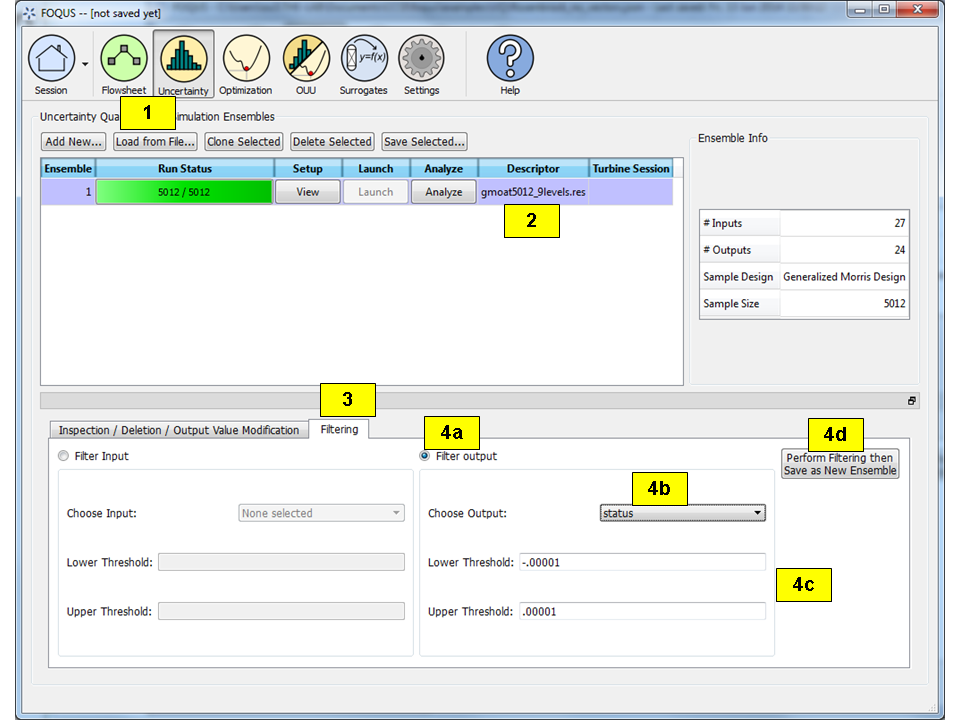
\includegraphics[width=6.5in,height=4in,keepaspectratio]{Chapt_uq/figs/tutorial/11_FilteringTab2}
		\caption{Data Manipulation, Filtering Tab}
		\label{fig:uqt_data_filter}
	\end{figure}
	\item{Select the file ``gmoat5012\_9levels.res'' in the examples\bs UQ folder. This
		file is an actual simulation ensemble that has already been run on the Turbine gateway.
		To find this file, the user may need to change the file filter to ``All files.''}
	\item{Select the \bu{Filtering} tab.}
	\item{Next, filtering the loaded simulation ensemble based on output values is performed. In particular,
		the user should keep only the samples in which the output parameter status is ``0.''}
	\begin{enumerate}
		\item{Select \textbf{\underline{Filter Output}}.}
		\item{Select ``status'' from the \textbf{\underline{Choose Output}} drop-down list.}
		\item{Enter -.00001 and .00001 as \textbf{\underline{Lower Threshold}} and \textbf{\underline{Upper Threshold}}
			respectively, and then click return within ``Lower threshold'' and ``Upper threshold.''}
		\item{Click \bu{Perform Filtering then Save as New Ensemble}.}
	\end{enumerate}
	\item{Once filtering is complete, a new row should be added to the
     simulation table (Figure \ref{fig:uqt_data_filter_results}). This
     ensemble contains only those samples that have a status value of
     ``0.'' Analysis can now be performed on this new ensemble because this
     ensemble contains only the valid simulations (i.e., those with output
     status value of 0), in which Aspen calculations have properly
     converged.
		%%% INSERT: Data Manipulation, Filtering Results
		\begin{figure}[H]
			\centering \includegraphics[width=6.5in,height=4in,keepaspectratio]{Chapt_uq/figs/tutorial/12_FilterResults2}
			\caption{Data Manipulation, Filtering Results}
			\label{fig:uqt_data_filter_results}
		\end{figure}
	}
\end{enumerate}

\subsubsection{Variable Deletion}
\label{subsubsec:uqt_vardel}

If an input or output variable is to be removed from consideration for
analysis, this can be done in the \bu{Inspection/Deletion/Output Value
  Modification} tab. Delete the status output from the previous filtering
as it is no longer needed for further analysis.
\begin{enumerate}
\item{Verify that the ensemble that resulted from filtering is selected. If not, select that ensemble.}
\item{Click the \bu{Inspection/Deletion/Output Modification} tab.}
\item{Scroll to the right of the table to the outputs, which are colored yellow.}
\item{Select the checkbox corresponding to the ``status'' output (the first output).}
\item{Click \bu{Perform Deletion then Save as New Ensemble}.}
\end{enumerate}
The results are illustrated in Figure \ref{fig:uqt_data_mod}. Note: The output count has decreased by one for the new ensemble. The user can verify that the ``status'' output was removed in the new ensemble by viewing this in the \textbf{\underline{Inspection/Deletion/Output Value Modification}} tab again. Deletion of an input can be performed similarly by selecting its checkbox and clicking the \textbf{\underline{Perform Deletion then Save as New Ensemble}} button.

%%% INSERT: Data Manipulation, Data / Output Value Modification Tab
\begin{figure}[H]
\centering 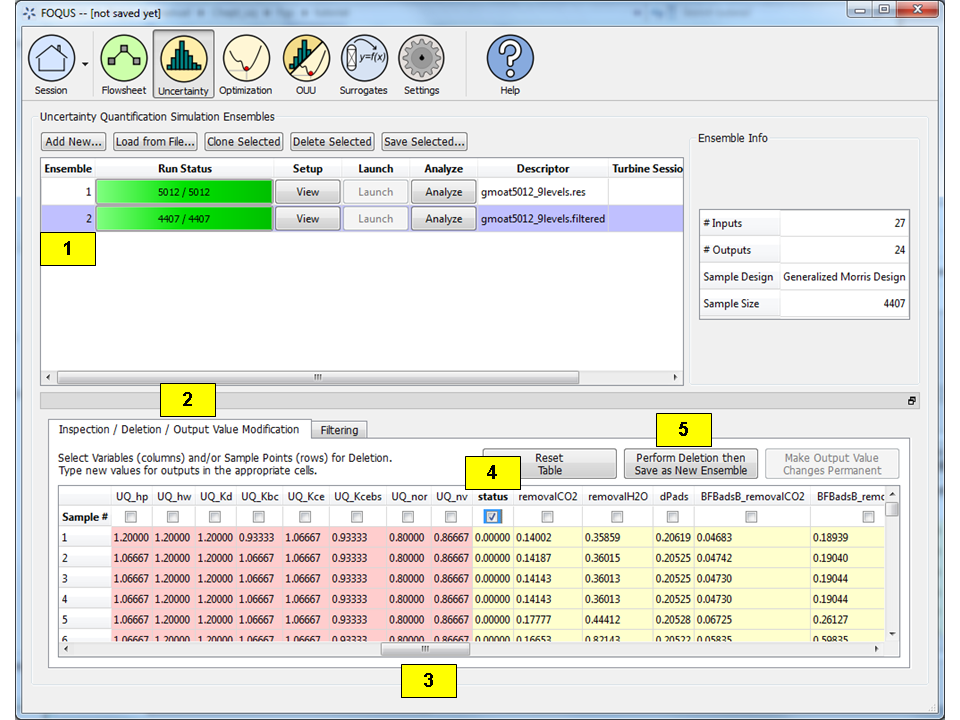
\includegraphics[width=6.5in,height=4in,keepaspectratio]{Chapt_uq/figs/tutorial/13_DataManipulation2}
\caption{Data Manipulation, Inspection/Deletion}
\label{fig:uqt_data_mod}
\end{figure}

\subsubsection{Output Value Modification}

To change the value of an output for a sample or several samples, follow steps below:
\begin{enumerate}
\item{Select an ensemble.}
\item{Click the \bu{Inspection/Deletion/Output Value Modification} tab.}
\item{Scroll to the right to the outputs.}
\item{Click on a cell for one of the outputs and enter a new value. Do the
  same for another cell. Notice that the modified cells turn green. This
  indicates the cells that have been modified.}
\item{Click \bu{Make Output Value Changes Permanent} to permanently change
  the values. The modified cells will turn yellow, indicating the permanent
  change. If the user wishes to reset the table and start over before
  making changes permanent, click the \bu{Reset Table}.}
\end{enumerate}

%%% INSERT: Data Manipulation, Output Value Modification
\begin{figure}[!htbp]
\centering \includegraphics[width=6.5in,height=4in,keepaspectratio]{Chapt_uq/figs/tutorial/14_DataManipulation_OutputModification2}
\caption{Data Manipulation, Value Modification}
\label{fig:uqt_data_mod_output}
\end{figure}

\pagebreak
